\begin{enumerate}
\item Let $A = \{1, 2, \{1, 2\}, b\}$ and let $B=\{a, b, \{1, 2\} \}$.
Find the following:
  \begin{enumerate}
  \item \wbitemsep $A \cap B$   \hint{ $ \{ b,  \{1, 2\} \} $ }
  \item \wbitemsep $A \cup B$ \hint{ $ \{1, 2, a, b, \{1, 2\} \} $ }
  \item \wbitemsep $A \setminus B$ \hint{  $ \{ 1, 2 \} $ }
  \item \wbitemsep $B \setminus A$ \hint{ $ \{ a \} $ }
  \item \wbitemsep $A \triangle B$ \hint{ $ \{ 1, 2, a \} $ }
  \end{enumerate}

\vfill


\workbookpagebreak

\item In a standard deck of playing cards one can distinguish sets
based on face-value and/or suit.  Let $A, 2, \ldots 9, 10, J, Q$ and $K$
represent the sets of cards having the various face-values.  Also, let
$\heartsuit$, $\spadesuit$, $\clubsuit$ and $\diamondsuit$ be the 
sets of cards having the possible suits.  Find the following
  \begin{enumerate}
  \item \wbitemsep$A \cap \heartsuit$ \hint{This is just the ace of hearts.}
  \item \wbitemsep$A \cup \heartsuit$ \hint{All of the hearts and the other three aces}
  \item \wbitemsep$J \cap (\spadesuit \cup \heartsuit)$ \hint{ These two cards are known as the one-eyed jacks.}
  \item \wbitemsep$K \cap \heartsuit$ \hint{The king of hearts, a.k.a. the suicide king.}
  \item \wbitemsep$A \cap K$ \hint{$\emptyset$ }
  \item \wbitemsep$A \cup K$ \hint{Eight cards: all four kings and all four aces.}
  \end{enumerate}

\vfill

%\textbookpagebreak
%\workbookpagebreak
%\hintspagebreak

\pagebreak

\item The following is a screenshot from the computational geometry program OpenSCAD (very hand for making models for 3-d printing\ldots)  In computational geometry we use the basice set operations together
with a few other types of transformations to create interesting models using simple components.  Across the top of the image below we see 3 sets of points in $\Reals^3$, a ball, a sort of 3-dimensional plus sign, and a disk.  Let's call the ball $A$, the plus sign $B$ and the disk $C$.   The nine shapes shown below them are made from $A$, $B$ and $C$ using union, intersection and set difference.  Identify them!

\vspace{.5in}
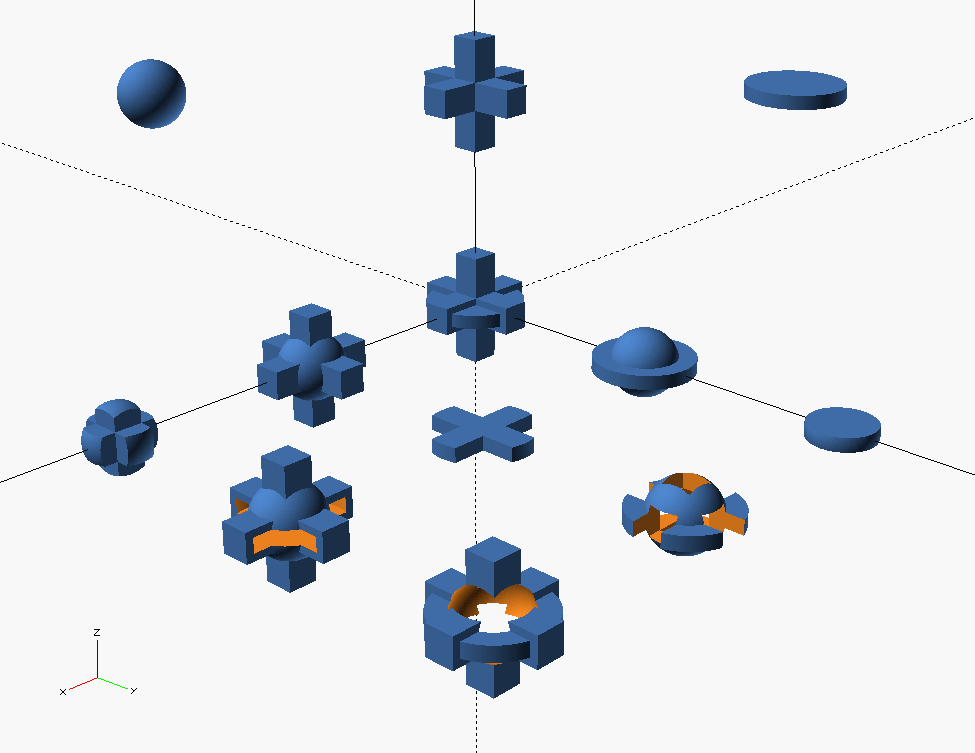
\includegraphics[scale=.375]{figures/set_ops.png}

\pagebreak

\item Do element-chasing proofs (show that an element is in the left-hand side if and only if it is in the right-hand side) to prove each of the following set equalities.  

  \begin{enumerate}
  \item \wbitemsep$\overline{A\cap B} \; = \; \overline{A}\cup\overline{B}$

  \item \wbitemsep$A\cup B \; = \; A\cup(\overline{A}\cap B)$

  \item \wbitemsep$A\triangle B \; = \; (A\cup B)\setminus(A\cap B)$

  \item \wbitemsep$(A\cup B)\setminus C \; = \; (A\setminus C)\cup(B\setminus C)$

  \end{enumerate}

\hint{Here's the first one (although I'm omiting justifications for each step.

\begin{gather*}
x \in \overline{A\cap B} \\
\iff \; {\lnot}(x \in A\cap B) \\
\iff \; {\lnot}(x \in A \; \land \; x \in B) \\
\iff \; {\lnot}(x \in A) \; \lor \; {\lnot}(x \in B) \\
\iff \; x \in \overline{A}  \; \lor \; x \in \overline{B} \\
\iff \; x \in \overline{A} \cup \overline{B}
\end{gather*}
}

\wbvfill

\workbookpagebreak

\item For each positive integer $n$, we'll define an interval $I_n$
by

\[ I_n = [-n, 1/n). \]

Find the union and intersection of all the intervals in this infinite family.

\[ \bigcup_{n \in \Naturals} I_n \quad = \]

\[ \bigcap_{n \in \Naturals} I_n \quad = \]

\hint{To better understand what is going on, first figure out what the first three or four
intervals actually are.

\[ I_1 \; = \; \underline{\rule{96pt}{0pt}} \]
\[ I_2 \; = \; \underline{\rule{96pt}{0pt}} \]
\[ I_3 \; = \; \underline{\rule{96pt}{0pt}} \]
\[ I_4 \; = \; \underline{\rule{96pt}{0pt}} \]

Any negative real number $r$ will be in the intersection only if  $r \geq -1$.  Certainly $0$ is in
the intersection since it is in each of the intervals.  Are there any positive numbers in the intersection?

In order to be in the union a real number just needs to be in {\em one} of the intervals.
}

\wbvfill

\workbookpagebreak

\item There is a set $X$ such that, for all sets $A$, we have 
$X \triangle A = A$.  What is $X$?

\wbvfill

\item There is a set $Y$ such that, for all sets $A$, we have 
$Y \triangle A = \overline{A}$.  What is $Y$?

\hint{One of the answers to the last two questions is $\emptyset$ and the other is $U$.  Decide
which is which.}

\wbvfill

\workbookpagebreak

\item In proving a set-theoretic identity, we are basically showing that
two sets are equal.  One reasonable way to proceed is to show that
each is contained in the other.  Prove that 
$A \cap (B \cup C) = (A \cap B) \cup (A \cap C)$ by showing that 
$A \cap (B \cup C) \subseteq (A \cap B) \cup (A \cap C)$ and 
$(A \cap B) \cup (A \cap C) \subseteq A \cap (B \cup C)$.

\wbvfill

\workbookpagebreak

\item Prove that 
$A \cup (B \cap C) = (A \cup B) \cap (A \cup C)$ by showing that 
$A \cup (B \cap C) \subseteq (A \cup B) \cap (A \cup C)$ and 
$(A \cup B) \cap (A \cup C) \subseteq A \cup (B \cap C)$.

\hint{This exercise, as well as the previous one, is really just about converting set-theoretic
statements into their logical equivalents, applying some rules of logic that we've already verified,
and then returning to a set-theoretic version of things.}

 \wbvfill

\workbookpagebreak
 
\item Prove the set-theoretic versions of DeMorgan's laws using the technique
discussed in the previous problems.

\wbvfill

\workbookpagebreak

\item The previous technique (showing that $A=B$ by arguing that
$A \subseteq B \; \land \; B \subseteq A$) will have an outline something like

\begin{proof} 
First we will show that $A \subseteq B$.\newline
Towards that end, suppose $x \in A$.

\begin{center}
$\vdots$
\end{center}

Thus $x \in B$.

Now, we will show that $B \subseteq A$. \newline
Suppose that $x \in B$.

\begin{center}
$\vdots$
\end{center}

Thus $x \in A$.

Therefore $A \subseteq B \; \land \; B \subseteq A$ so we conclude that $A=B$.
\end{proof}

Formulate a proof that $A \triangle B \; = \; (A \cup B) \setminus (A \cap B)$ that follows this outline.

\hint{The definition of $A \triangle B$ is $(A\setminus B) \cup (B\setminus A)$.  The definition of 
$X \setminus Y$ is $X \cap \overline{Y}$.   Restating things in terms of $\cap$ and $\cup$ (and complementation) should help.  So your first few lines should be:

 \begin{quote} 
 Suppose $x \in  A \triangle B$.  
 
Then, by definition, $x \in (A\setminus B) \cup (B\setminus A)$.
 
 So, $x \in (A \cap \overline{B}) \cup (B \cap \overline{A})$.
   
\begin{center}
$\vdots$
\end{center}

\end{quote}
}

\wbvfill

\workbookpagebreak

\end{enumerate}


%% Emacs customization
%% 
%% Local Variables: ***
%% TeX-master: "GIAM-hw.tex" ***
%% comment-column:0 ***
%% comment-start: "%% "  ***
%% comment-end:"***" ***
%% End: ***

